\documentclass[12pt]{article}

\usepackage{fullpage,amsmath,amssymb,amsthm,graphicx}

\newcommand{\D}{\displaystyle}

\title{Math 199 CD2: More on Derivative}
\date{\today}


\begin{document}
	
	\maketitle
	
	\begin{enumerate}
		\item Find the derivative of the following functions: 
		\begin{enumerate}
			\item $$f(x)=\left(\frac{x \sqrt[4] x}{x^{1/6}}\right)^{12}+\ln\left(\frac{\pi^3}{e^2+4}\right)$$
			
			\vskip 4cm
			
			\item $$f(x)=8x^{-5/6}+\frac{10^{10}}{x^{-9/2}}$$
			
			\vskip 4cm
			\item $f(x) = (2x -3)^2$. Just some simple chain rule to get you started
		\end{enumerate}
	\newpage
	
		\item At what points does the normal line (perpendicular line) to the curve $y = x^2 - 3x + 5$ at the point $(3, 5)$ 	intersect the curve?. Hint: the product of the slopes of 2 perpendicular lines should be $-1$. So find the formula for the normal line first  \\
		
		\vskip 7cm
		\item Find the point(s) on the graph of $y = x^2$ at which the tangent line passes through $(2, -12)$
		
		\vskip 7cm
		
		\item Find the point(s) on the graph of $y = x^2$ at which the tangent line is parallel to the line $y= 6x -1$. Hint: 2 lines are parallel must have the same slope
		
		\vskip 7cm
		
		\item We haven't talked much about the second derivative but it's super useful for visualizing the function. The second derivative tells you whether the function is concave up (if positive) or down (if negative) at a certain point.\\ 
		If, for all $x$, $f'(x)>0$ and $f''(x)<0$, which of the curves below could be part of the graph of $f$? Hint: \\
		
		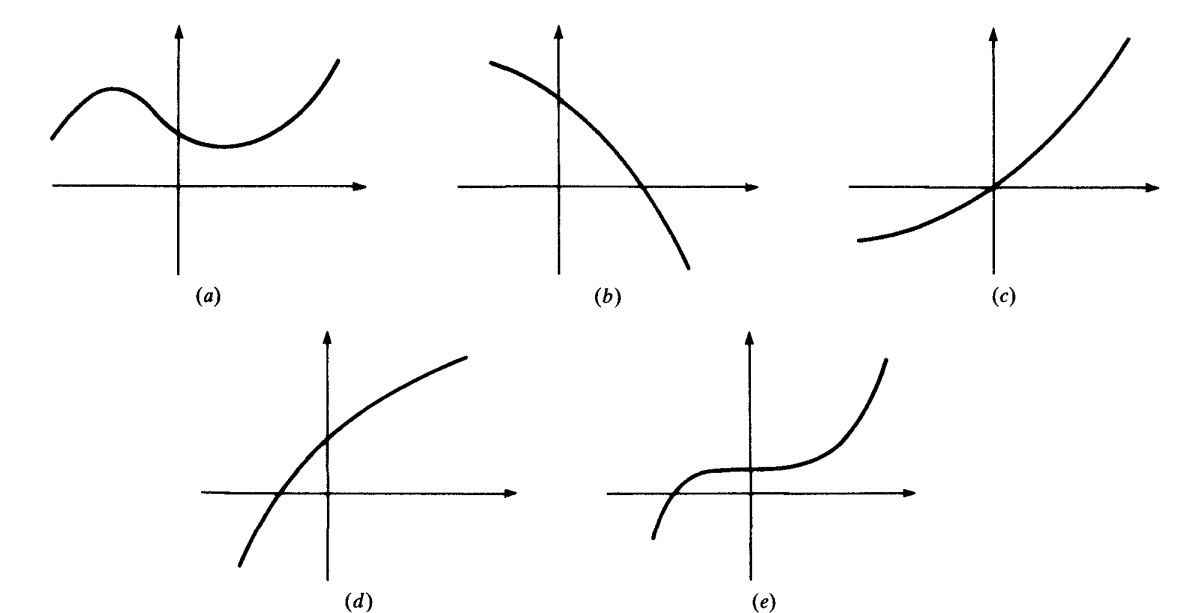
\includegraphics[scale=0.6]{p6.png}
	\end{enumerate}
	
	
	

	
\end{document}